%!TeX program = xelatex

% Define document font, paper size and type %
\documentclass[12pt,a4paper,numbers=noenddot]{scrreprt}

% Include all auxiliary packages
% All required packages to be used within this project

% Margin definitions
\usepackage[a4paper,vmargin=3cm,hmargin=3cm]{geometry}

% Packages to be used
\usepackage{fontspec}
\usepackage{eurosym}
\usepackage{amssymb}
\usepackage{mathtools}
\usepackage{amsmath}
\usepackage{upquote}
\usepackage{microtype}
\usepackage{longtable,booktabs}
\usepackage{graphicx}
\usepackage{grffile}
\usepackage{appendix}
\usepackage{float}
\usepackage{pst-all}
\usepackage{geometry}
\usepackage{xcolor}
\usepackage{xpatch}
\usepackage{nccmath}
\usepackage{subcaption}
\usepackage{xcolor}
\usepackage{multirow}
\usepackage{setspace}
\usepackage{bm}
\usepackage[
  starfontserif % comment for sans glyphs
]{starfont}
\captionsetup{compatibility=false}
\usepackage[crop=off]{auto-pst-pdf}
\usepackage[normalem]{ulem}

% Custom links color
\definecolor{linkscolor}{rgb}{0.89, 0.26, 0.2}

\usepackage[unicode=true,bookmarks=true,bookmarksopen=false,
  bookmarksopenlevel=1,pdfborder={0 0 0},backref=false,
  colorlinks=true,allcolors=red,pdfstartview=Fit,
  pdfcenterwindow=true,pdfdisplaydoctitle=true,
  pdfpagelayout=OneColumn,linktocpage=true]{hyperref}
\useunder{\uline}{\ul}{}

% Path for all graphic utilities
\graphicspath{{fig/}}



% Bibliography setup
\usepackage[backend=biber, style=ieee, citestyle=authoryear, sorting=ynt]{biblatex}
\bibliography{bib/articles_modern}
\bibliography{bib/books_classic}
\bibliography{bib/books_modern}

% Custom commands: always the last ones to import to properly override default
% Custom paragraph distance
\setlength{\parskip}{1em plus 2pt minus 1pt}
\setlength{\emergencystretch}{3em}

% Beautiful captions for figures
\captionsetup[figure]{
  format=hang,
  name=Fig.,
  singlelinecheck=off,
  labelsep=colon,
  labelfont=bf,
  font=small
}

% Improve quotations
\newcommand{\quoteauthor}[2]
{
  \begin{flushright}
    \rightskip=1.8cm\textit{``{#1}''} \\
    \vspace{.2em}
    \rightskip=.8cm---{#2}
  \end{flushright}
}

% Improve hyperlinks when citing references
\DeclareCiteCommand{\citetitle}
{\boolfalse{citetracker}%
  \boolfalse{pagetracker}%
  \usebibmacro{prenote}}
{\ifciteindex
  {\indexfield{indextitle}}
  {}%
  \printtext[bibhyperref]{\printfield[citetitle]{labeltitle}}}
{\multicitedelim}
{\usebibmacro{postnote}}

\DeclareCiteCommand{\cite}
{\usebibmacro{prenote}}
{\usebibmacro{citeindex}%
  \printtext[bibhyperref]{\usebibmacro{cite}}}
{\multicitedelim}
{\usebibmacro{postnote}}

\DeclareCiteCommand*{\cite}
{\usebibmacro{prenote}}
{\usebibmacro{citeindex}%
  \printtext[bibhyperref]{\usebibmacro{citeyear}}}
{\multicitedelim}
{\usebibmacro{postnote}}

\DeclareCiteCommand{\parencite}[\mkbibparens]
{\usebibmacro{prenote}}
{\usebibmacro{citeindex}%
  \printtext[bibhyperref]{\usebibmacro{cite}}}
{\multicitedelim}
{\usebibmacro{postnote}}

\DeclareCiteCommand*{\parencite}[\mkbibparens]
{\usebibmacro{prenote}}
{\usebibmacro{citeindex}%
  \printtext[bibhyperref]{\usebibmacro{citeyear}}}
{\multicitedelim}
{\usebibmacro{postnote}}

\DeclareCiteCommand{\footcite}[\mkbibfootnote]
{\usebibmacro{prenote}}
{\usebibmacro{citeindex}%
  \printtext[bibhyperref]{ \usebibmacro{cite}}}
{\multicitedelim}
{\usebibmacro{postnote}}

\DeclareCiteCommand{\footcitetext}[\mkbibfootnotetext]
{\usebibmacro{prenote}}
{\usebibmacro{citeindex}%
  \printtext[bibhyperref]{\usebibmacro{cite}}}
{\multicitedelim}
{\usebibmacro{postnote}}

\DeclareCiteCommand{\textcite}
{\boolfalse{cbx:parens}}
{\usebibmacro{citeindex}%
  \printtext[bibhyperref]{\usebibmacro{textcite}}}
{\ifbool{cbx:parens}
  {\bibcloseparen\global\boolfalse{cbx:parens}}
  {}%
  \multicitedelim}
{\usebibmacro{textcite:postnote}}

\DeclareCiteCommand{\citeauthor}%
{\boolfalse{citetracker}%
  \boolfalse{pagetracker}%
  \usebibmacro{prenote}}
{\ifciteindex
  {\indexnames{labelname}}
  {}%
  \printtext[bibhyperref]{\printnames{labelname}}}
{\multicitedelim}
{\usebibmacro{postnote}}

% Reduce top and lower space in equations
\xpatchcmd{\NCC@ignorepar}{%
  \abovedisplayskip\abovedisplayshortskip}
{%
  \abovedisplayskip\abovedisplayshortskip%
  \belowdisplayskip\belowdisplayshortskip}
{}{}

% Do not restart footnotes counter
\counterwithout{footnote}{chapter}

% Custom norm for equations
\DeclarePairedDelimiter{\norm}{\lVert}{\rVert}

% Custom arctan2 and atan2 functions
\DeclareMathOperator{\arctantwo}{arctan2}
\DeclareMathOperator{\atantwo}{atan2}

% Custom piecewise functions
\DeclarePairedDelimiter\Floor\lfloor\rfloor
\DeclarePairedDelimiter\Ceil\lceil\rceil

% Trigonometric functions
\DeclareMathOperator{\sech}{sech}
\DeclareMathOperator{\csch}{csch}
\DeclareMathOperator{\arcsec}{arcsec}
\DeclareMathOperator{\arccot}{arccot}
\DeclareMathOperator{\arccsc}{arccsc}
\DeclareMathOperator{\arccosh}{arccosh}
\DeclareMathOperator{\arcsinh}{arcsinh}
\DeclareMathOperator{\arctanh}{arctanh}
\DeclareMathOperator{\arcsech}{arcsech}
\DeclareMathOperator{\arccsch}{arccsch}
\DeclareMathOperator{\arccoth}{arccoth}

% Custom command for blank page
\newcommand{\blankpage}{\newpage \ \thispagestyle{empty} \newpage}

% Custom command for the table of contents
\newcommand{\maketableofcontents}{\tableofcontents \blankpage \listoffigures \blankpage \listoftables \blankpage}

% Solar System Symbols
\DeclareSymbolFont{starfontsym}{OT1}{sts}{m}{n}
\DeclareMathSymbol{\mathSun}{\mathord}{starfontsym}{115}
\DeclareMathSymbol{\mathMercury}{\mathord}{starfontsym}{102}
\DeclareMathSymbol{\mathVenus}{\mathord}{starfontsym}{103}
\DeclareMathSymbol{\mathTerra}{\mathord}{starfontsym}{76}
\DeclareMathSymbol{\mathvarTerra}{\mathord}{starfontsym}{108}
\DeclareMathSymbol{\mathMoon}{\mathord}{starfontsym}{100}
\DeclareMathSymbol{\mathvarMoon}{\mathord}{starfontsym}{97}
\DeclareMathSymbol{\mathMars}{\mathord}{starfontsym}{104}
\DeclareMathSymbol{\mathJupiter}{\mathord}{starfontsym}{106}
\DeclareMathSymbol{\mathSaturn}{\mathord}{starfontsym}{83}
\DeclareMathSymbol{\mathUranus}{\mathord}{starfontsym}{70}
\DeclareMathSymbol{\mathvarUranus}{\mathord}{starfontsym}{65}
\DeclareMathSymbol{\mathNeptune}{\mathord}{starfontsym}{71}
\DeclareMathSymbol{\mathPluto}{\mathord}{starfontsym}{74}
\DeclareMathSymbol{\mathvarPluto}{\mathord}{starfontsym}{72}


% Start the document
\begin{document}

% Switch off page numbering %
\pagenumbering{Roman}

% Append cover and prologue to actual document %
% Start generating the title page
\begin{titlepage}

  % All content will be centered within this page
  \begin{center}

    % Add cover logo
    \begin{figure}[h]
      \centering
      
\includegraphics[width=\linewidth]{static/banner.png}
    \end{figure}
    \vspace{1cm}

    % Nature of the document
    \textsc{\large
      UNIVERSIDAD INTERNACIONAL DE VALENCIA
    }\\[0.25cm]
    \textsc{\large
      Master in Astronomy and Astrophysics \\
      Academic year 2023-2024
    }\\[1cm]
    \textsc{\large
      \textit{Segunda convocatoria}
    }\\[1.25cm]

    % Title of the essay
    \noindent\rule{\textwidth}{1pt}
    \\[0.25cm]
    {
    % Apply font size and color
    \fontsize{35pt}{35pt}\selectfont
    {
      Interstellar Interceptors. Mission design for rendezvous with objects in hyperbolic orbits.
    }
    }
    \noindent\rule{\textwidth}{1pt}

    \vspace{1.5cm}
    \textsc{\Large
      Jorge Martínez Garrido
    }\\[1.25cm]
    \textsc{\large
      Supervised by:
    }\\[0.25cm]
    \textsc{\large
      Josep M. Trigo-Rodríguez (ICE-CSIC/IEEC) \\
      Eloy Peña-Asensio (Politecnico di Milano)
    }\\[1.5cm]

    \textsc{\large
      April, 2024
    }\\[0.25cm]
    \textsc{\large
      Madrid, Spain
    }\\[0.25cm]

  \end{center}
\end{titlepage}

\blankpage
\chapter*{Abstract}

This research offers a thorough examination of transfer orbits specifically
tailored for intercepting interstellar visitors. Through an exhaustive analysis
of diverse launch scenarios, detailed porkchop plots are crafted to illustrate
the specific energy required at launch for both prograde and retrograde
transfers. Additionally, isolines delineating the total time of flight and
velocity upon arrival are meticulously calculated across a broad spectrum of
launch and arrival dates. These efforts enable the precise determination of
optimal energy transfer paths. Departure strategies from Earth, Lagrange point
L2, and gravity-assisted maneuvers are thoroughly explored, providing insights
into their efficacy.

The study's outcomes harmonize with established mission proposals, exemplified
by the Comet Interceptor, corroborating the strategic significance of Lagrange
point L2 as a launch locus for interstellar missions. This underscores the
imperative for enhancing surveillance research initiatives centered on
identifying interlopers and fortifying pre-planned missions stationed at
Lagrange point L2. Given the validated efficacy of L2 as a launch platform,
heightened emphasis on surveillance research emerges as essential, ensuring
preparedness to capitalize on evolving opportunities for celestial exploration
and scientific inquiry.


\vspace{4cm}
\textbf{Keywords:} Interlopers, transfer orbits, porkchop plots, Lagrange points,
gravity-assisted maneuvers, interstellar missions, surveillance research,
mission design, celestial exploration

\blankpage

% Start the table of contents, figures and tables %
\maketableofcontents

% ---------- BEGIN OF CONTENT FILES -------------

% --------------------------------- %
% --- INTRODUCTION TO THIS WORK --- %
% --------------------------------- %
\chapter{Introduction to this work}
\pagenumbering{arabic}

The initial chapter is dedicated to introducing fundamental concepts pertinent
to the addressed problem, delineating the various methodologies employed and
outlining the objectives attained. These components serve to enhance the
reader's comprehension of the project's framework. Furthermore, the concluding
sections offer a compilation of real-world applications alongside a concise
socioeconomic evaluation, aiming to substantiate the contemporary relevance and
significance of the problem at hand.

% --- Sections for this chapter --- %
\section{Problem description and motivation}

The discovery of interstellar objects such as 'Oumuamua and Borisov within our
solar system has ignited a surge of curiosity and scientific interest. These
sub-kilometer-sized visitors, originating from distant stellar systems, present
a unique opportunity to study extraterrestrial bodies that have traversed vast
cosmic distances. Therefore, the main motivation behind the study of these
objects are:

\begin{itemize}

  \item \textbf{Better understanding the formation of planetary systems.}
        Interstellar objects can provide insights into the formation and
        dynamics of planetary systems beyond our own. This could help to
        confirm or reject the Nebular hyphotesis, which is the most popular
        model proposed for the formation of planetary systems.

  \item \textbf{Exploring the origins of life.} Analyzing the composition of
        interstellar objects could provide valuable information about the
        chemical and physical conditions present in other planetary
        systems, shedding light on the origins of life in the universe, which
        could support or reject the panspermia hyphotesis.

  \item \textbf{Technological innovation.} By pushing the technological
        boundaries of space exploration, missions to intercept interstellar
        objects could lead to the development of new propulsion systems and
        spacecraft capable of reaching unprecedented speeds and distances.

\end{itemize}

Given their exceptionally high eccentricities, heliocentric velocities, and
fleeting passage through the planetary region, there is a pressing need for the
development of ready-to-launch missions capable of intercepting them.

However, the design of such missions is not straightforward. The high velocities
of these objects, combined with their limited observation windows, make it
difficult to accurately predict their trajectories and plan for rendezvous
within the short timeframes available.

This problem presents the main motivation of this work: \textbf{devising mission
orbits capable of intercepting interstellar objects}.

This research stems from the desire to unlock the mysteries surrounding these
enigmatic interstellar travelers, gathering invaluable data or even returning
samples from their surfaces. This pursuit not only promises to broaden our
understanding of celestial dynamics and planetary formation but also holds
profound implications for the future of space exploration and our comprehension
of the broader universe.

\section{Objectives and goals}

The main objetive of this project is to devise suitable targetting orbits for
interstellar ojects. To achieve this purpose, the whole process is divided
into the following key objectives:

\begin{itemize}

    \item \textbf{Research on interstellar objects.}
        The definition of interstellar object is presented together with the
        official IAU nomenclature. The only two discovered objects,
        'Oumuamua and Borisov, are presented together with their main
        characteristics. The importance of the solar apex is explained
        too.

    \item \textbf{Research on targetting orbits.}
        The main types of targetting orbits are presented, together with their
        main characteristics. The main differences between them are explained
        and the main advantages and disadvantages of each type are presented.

\end{itemize}

\section{Social and economic impact}

Public scrutiny often targets science funding, demanding evidence of its
tangible social and economic benefits. This challenge is particularly pronounced
in fields like astronomy and astrodynamics, where justifying investments for
exploring distant celestial objects and phenomena is difficult.

A pivotal outcome of the research process lies in the array of technologies
conceived, subsequently finding diverse applications for societal improvement.
Consider the iconic Apollo program as an example. The groundbreaking
technologies developed for the success of Apollo missions, including the
formidable Saturn V rocket, the versatile Lunar Module, and the pioneering
Apollo Guidance Computer (AGC) depicted in Figure \ref{fig:apollo-agc}, have
transcended their original purposes and found invaluable utility across various
fields.

\begin{figure}[H]
  \centering
  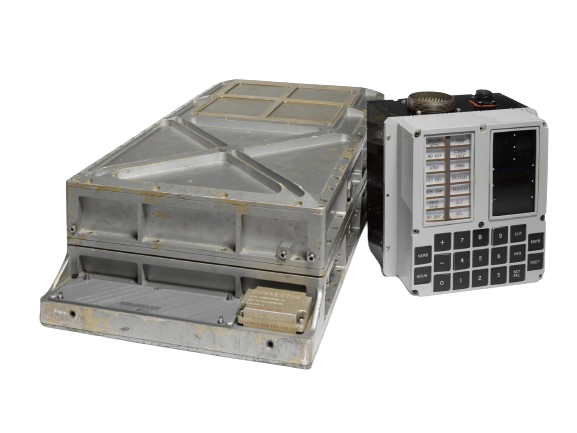
\includegraphics[width=0.7\textwidth]{static/apollo-agc.png}
  \caption[Apollo Guidance Computer]{
  The figure displays two key components of the AGC: the Computer Unit,
  constructed entirely from NOR gate integrated circuits on the left, and
  the Display and Keyboard (DSKY) on the right, used by astronauts to
  interact with the AGC.
  }
  \label{fig:apollo-agc}
\end{figure}

These technologies incorporated novel approaches, notably the utilization of
integrated circuits (ICs). The challenges addressed during this era have paved
the way for modern advancements, evident in the widespread adoption of
fly-by-wire technology in commercial airplanes and the ubiquitous presence of
ICs in various devices.

Similarly, the study of interstellar objects holds promise for fostering
innovation in propulsion, navigation, and observation technologies. These
advancements can be subsequently adapted and applied in other disciplines, such
as Earth observation, satellite communications, and space debris mitigation.



% ----------- END OF CONTENT FILES -------------


% Cite the bibliography
\printbibliography

\end{document}
